% Options for packages loaded elsewhere
\PassOptionsToPackage{unicode}{hyperref}
\PassOptionsToPackage{hyphens}{url}
\PassOptionsToPackage{dvipsnames,svgnames,x11names}{xcolor}
%
\documentclass[
  letterpaper,
  DIV=11,
  numbers=noendperiod,
  oneside]{scrartcl}

\usepackage{amsmath,amssymb}
\usepackage{iftex}
\ifPDFTeX
  \usepackage[T1]{fontenc}
  \usepackage[utf8]{inputenc}
  \usepackage{textcomp} % provide euro and other symbols
\else % if luatex or xetex
  \usepackage{unicode-math}
  \defaultfontfeatures{Scale=MatchLowercase}
  \defaultfontfeatures[\rmfamily]{Ligatures=TeX,Scale=1}
\fi
\usepackage{lmodern}
\ifPDFTeX\else  
    % xetex/luatex font selection
\fi
% Use upquote if available, for straight quotes in verbatim environments
\IfFileExists{upquote.sty}{\usepackage{upquote}}{}
\IfFileExists{microtype.sty}{% use microtype if available
  \usepackage[]{microtype}
  \UseMicrotypeSet[protrusion]{basicmath} % disable protrusion for tt fonts
}{}
\makeatletter
\@ifundefined{KOMAClassName}{% if non-KOMA class
  \IfFileExists{parskip.sty}{%
    \usepackage{parskip}
  }{% else
    \setlength{\parindent}{0pt}
    \setlength{\parskip}{6pt plus 2pt minus 1pt}}
}{% if KOMA class
  \KOMAoptions{parskip=half}}
\makeatother
\usepackage{xcolor}
\usepackage[top=30mm,bottom=30mm,left=15mm,right=80mm,marginparwidth=60mm,marginparsep=10mm,heightrounded]{geometry}
\setlength{\emergencystretch}{3em} % prevent overfull lines
\setcounter{secnumdepth}{-\maxdimen} % remove section numbering
% Make \paragraph and \subparagraph free-standing
\makeatletter
\ifx\paragraph\undefined\else
  \let\oldparagraph\paragraph
  \renewcommand{\paragraph}{
    \@ifstar
      \xxxParagraphStar
      \xxxParagraphNoStar
  }
  \newcommand{\xxxParagraphStar}[1]{\oldparagraph*{#1}\mbox{}}
  \newcommand{\xxxParagraphNoStar}[1]{\oldparagraph{#1}\mbox{}}
\fi
\ifx\subparagraph\undefined\else
  \let\oldsubparagraph\subparagraph
  \renewcommand{\subparagraph}{
    \@ifstar
      \xxxSubParagraphStar
      \xxxSubParagraphNoStar
  }
  \newcommand{\xxxSubParagraphStar}[1]{\oldsubparagraph*{#1}\mbox{}}
  \newcommand{\xxxSubParagraphNoStar}[1]{\oldsubparagraph{#1}\mbox{}}
\fi
\makeatother


\providecommand{\tightlist}{%
  \setlength{\itemsep}{0pt}\setlength{\parskip}{0pt}}\usepackage{longtable,booktabs,array}
\usepackage{calc} % for calculating minipage widths
% Correct order of tables after \paragraph or \subparagraph
\usepackage{etoolbox}
\makeatletter
\patchcmd\longtable{\par}{\if@noskipsec\mbox{}\fi\par}{}{}
\makeatother
% Allow footnotes in longtable head/foot
\IfFileExists{footnotehyper.sty}{\usepackage{footnotehyper}}{\usepackage{footnote}}
\makesavenoteenv{longtable}
\usepackage{graphicx}
\makeatletter
\def\maxwidth{\ifdim\Gin@nat@width>\linewidth\linewidth\else\Gin@nat@width\fi}
\def\maxheight{\ifdim\Gin@nat@height>\textheight\textheight\else\Gin@nat@height\fi}
\makeatother
% Scale images if necessary, so that they will not overflow the page
% margins by default, and it is still possible to overwrite the defaults
% using explicit options in \includegraphics[width, height, ...]{}
\setkeys{Gin}{width=\maxwidth,height=\maxheight,keepaspectratio}
% Set default figure placement to htbp
\makeatletter
\def\fps@figure{htbp}
\makeatother
% definitions for citeproc citations
\NewDocumentCommand\citeproctext{}{}
\NewDocumentCommand\citeproc{mm}{%
  \begingroup\def\citeproctext{#2}\cite{#1}\endgroup}
\makeatletter
 % allow citations to break across lines
 \let\@cite@ofmt\@firstofone
 % avoid brackets around text for \cite:
 \def\@biblabel#1{}
 \def\@cite#1#2{{#1\if@tempswa , #2\fi}}
\makeatother
\newlength{\cslhangindent}
\setlength{\cslhangindent}{1.5em}
\newlength{\csllabelwidth}
\setlength{\csllabelwidth}{3em}
\newenvironment{CSLReferences}[2] % #1 hanging-indent, #2 entry-spacing
 {\begin{list}{}{%
  \setlength{\itemindent}{0pt}
  \setlength{\leftmargin}{0pt}
  \setlength{\parsep}{0pt}
  % turn on hanging indent if param 1 is 1
  \ifodd #1
   \setlength{\leftmargin}{\cslhangindent}
   \setlength{\itemindent}{-1\cslhangindent}
  \fi
  % set entry spacing
  \setlength{\itemsep}{#2\baselineskip}}}
 {\end{list}}
\usepackage{calc}
\newcommand{\CSLBlock}[1]{\hfill\break\parbox[t]{\linewidth}{\strut\ignorespaces#1\strut}}
\newcommand{\CSLLeftMargin}[1]{\parbox[t]{\csllabelwidth}{\strut#1\strut}}
\newcommand{\CSLRightInline}[1]{\parbox[t]{\linewidth - \csllabelwidth}{\strut#1\strut}}
\newcommand{\CSLIndent}[1]{\hspace{\cslhangindent}#1}

\usepackage{lastpage}
        \usepackage{fancyhdr}
        \usepackage{titling}
        \pagestyle{fancy}
        \fancyhead[L]{CMPE2150 PCB Project X}
        \fancyhead[R]{KiCAD Makeup Assignment}
        \fancyfoot[C]{\thepage/\pageref*{LastPage}}
        \setlength{\droptitle}{-2cm}
        
\KOMAoption{captions}{tablesignature}
\makeatletter
\@ifpackageloaded{tcolorbox}{}{\usepackage[skins,breakable]{tcolorbox}}
\@ifpackageloaded{fontawesome5}{}{\usepackage{fontawesome5}}
\definecolor{quarto-callout-color}{HTML}{909090}
\definecolor{quarto-callout-note-color}{HTML}{0758E5}
\definecolor{quarto-callout-important-color}{HTML}{CC1914}
\definecolor{quarto-callout-warning-color}{HTML}{EB9113}
\definecolor{quarto-callout-tip-color}{HTML}{00A047}
\definecolor{quarto-callout-caution-color}{HTML}{FC5300}
\definecolor{quarto-callout-color-frame}{HTML}{acacac}
\definecolor{quarto-callout-note-color-frame}{HTML}{4582ec}
\definecolor{quarto-callout-important-color-frame}{HTML}{d9534f}
\definecolor{quarto-callout-warning-color-frame}{HTML}{f0ad4e}
\definecolor{quarto-callout-tip-color-frame}{HTML}{02b875}
\definecolor{quarto-callout-caution-color-frame}{HTML}{fd7e14}
\makeatother
\makeatletter
\@ifpackageloaded{caption}{}{\usepackage{caption}}
\AtBeginDocument{%
\ifdefined\contentsname
  \renewcommand*\contentsname{Table of contents}
\else
  \newcommand\contentsname{Table of contents}
\fi
\ifdefined\listfigurename
  \renewcommand*\listfigurename{List of Figures}
\else
  \newcommand\listfigurename{List of Figures}
\fi
\ifdefined\listtablename
  \renewcommand*\listtablename{List of Tables}
\else
  \newcommand\listtablename{List of Tables}
\fi
\ifdefined\figurename
  \renewcommand*\figurename{Figure}
\else
  \newcommand\figurename{Figure}
\fi
\ifdefined\tablename
  \renewcommand*\tablename{Table}
\else
  \newcommand\tablename{Table}
\fi
}
\@ifpackageloaded{float}{}{\usepackage{float}}
\floatstyle{ruled}
\@ifundefined{c@chapter}{\newfloat{codelisting}{h}{lop}}{\newfloat{codelisting}{h}{lop}[chapter]}
\floatname{codelisting}{Listing}
\newcommand*\listoflistings{\listof{codelisting}{List of Listings}}
\makeatother
\makeatletter
\makeatother
\makeatletter
\@ifpackageloaded{caption}{}{\usepackage{caption}}
\@ifpackageloaded{subcaption}{}{\usepackage{subcaption}}
\makeatother
\makeatletter
\@ifpackageloaded{sidenotes}{}{\usepackage{sidenotes}}
\@ifpackageloaded{marginnote}{}{\usepackage{marginnote}}
\makeatother

\ifLuaTeX
  \usepackage{selnolig}  % disable illegal ligatures
\fi
\usepackage{bookmark}

\IfFileExists{xurl.sty}{\usepackage{xurl}}{} % add URL line breaks if available
\urlstyle{same} % disable monospaced font for URLs
\hypersetup{
  pdftitle={CMPE2150 PCB Project X},
  pdfauthor={AJ Armstrong},
  colorlinks=true,
  linkcolor={blue},
  filecolor={Maroon},
  citecolor={Blue},
  urlcolor={Blue},
  pdfcreator={LaTeX via pandoc}}


\title{CMPE2150 PCB Project X}
\usepackage{etoolbox}
\makeatletter
\providecommand{\subtitle}[1]{% add subtitle to \maketitle
  \apptocmd{\@title}{\par {\large #1 \par}}{}{}
}
\makeatother
\subtitle{KiCAD Makeup Assignment}
\author{AJ Armstrong}
\date{17 May 2025}

\begin{document}
\maketitle

\renewcommand*\contentsname{Table of contents}
{
\hypersetup{linkcolor=}
\setcounter{tocdepth}{3}
\tableofcontents
}

\begin{tcolorbox}[enhanced jigsaw, toptitle=1mm, colbacktitle=quarto-callout-important-color!10!white, colframe=quarto-callout-important-color-frame, bottomtitle=1mm, colback=white, opacityback=0, coltitle=black, opacitybacktitle=0.6, rightrule=.15mm, titlerule=0mm, arc=.35mm, title=\textcolor{quarto-callout-important-color}{\faExclamation}\hspace{0.5em}{Important}, leftrule=.75mm, breakable, toprule=.15mm, bottomrule=.15mm, left=2mm]

You should already have completed an exercise introducing and exploring
KiCAD 9.0 and worked on the CMPE2150 PCB Project. This project is a
similar but smaller version of the that one, suitable for a skills check
or timed exam. It assumes your familiarity with those exercises and
notes and will therefore be comparatively terse. See the original
project if you need more clarity on specific tasks. The steps in this
exercise are broadly the same and presented in the same order as the
original project.

\end{tcolorbox}

\newpage{}

\subsection{Part 1 - Schematic
Capture}\label{part-1---schematic-capture}

\subsubsection{The Circuit Design---Programmable Pulse
Generator}\label{the-circuit-designprogrammable-pulse-generator}

The circuit we have selected for you to realize is shown below.

\begin{figure}[H]

\sidecaption{Programmable Pulse Generator}

{\centering 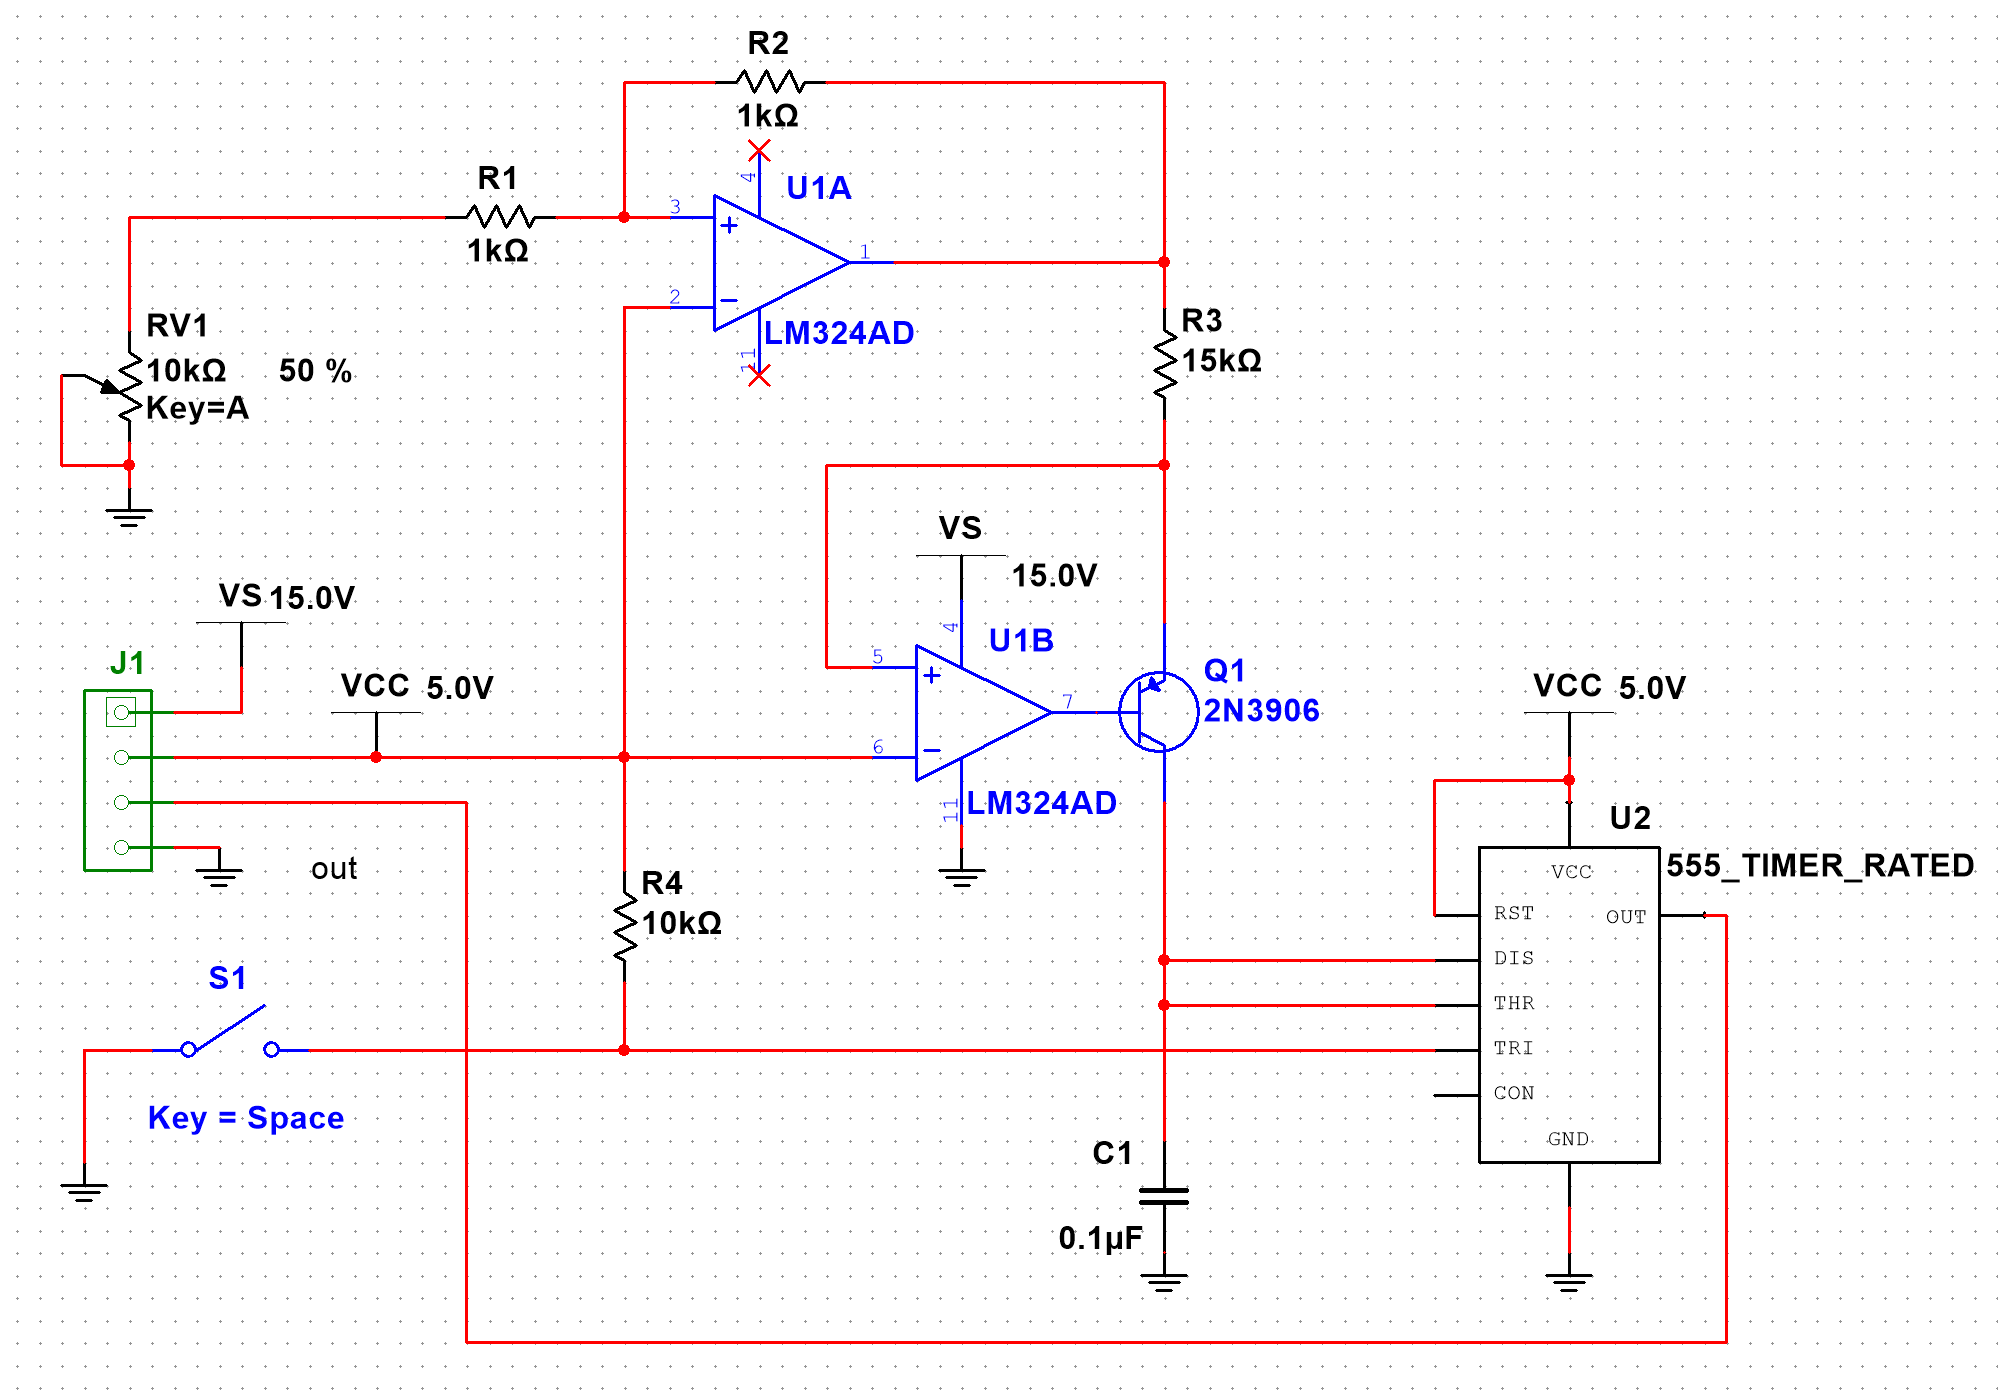
\includegraphics{images/pulsegenschem.png}

}

\end{figure}%

This circuit is from the classic \emph{The Art of Electronics} {[}1, p.
242{]}\marginpar{\begin{footnotesize}
\begin{CSLReferences}{2}{0}
\bibitem[\citeproctext]{ref-AoE3}
\CSLLeftMargin{{[}1{]} }%
\CSLRightInline{P. Horowitz and W. Hill, \emph{The art of electronics},
3rd ed. Cambridge University Press, 2015.}
\end{CSLReferences}
\vspace{2mm}\par\end{footnotesize}}.
It is a variable width single pulse generator. The potentiometer sets
the duration of the pulse and the switch triggers it.

The four-pin header represents the board's inputs and outputs:

\begin{itemize}
\item
  \(V_S\) is the voltage source to power the op amps (the top rail). It
  will ordinarily be \(+15V_{DC}\).
\item
  \(V_{cc}\) is the voltage source for the 555 timer and also serves as
  the ``on'' digital voltage reference. It will be \(+5V_{DC}\).
\item
  \(Out\) is the output of the timer. This is where the pulse generated
  by the circuit appears.
\item
  \(Gnd\) is the ground reference for the other three pins.
\end{itemize}

\newpage{}

\subsubsection{A - KiCAD Project Setup}\label{a---kicad-project-setup}

Follow the procedure below---nearly identical to the detailed one
presented in the tutorial---to create your project to realize the
schematic above.

\begin{enumerate}
\def\labelenumi{\arabic{enumi}.}
\item
  Open KiCAD 9.0 and select \emph{File → New Project}. Name your project
  ``PulseGenerator-\emph{\textless UserID\textgreater{}}'', replacing
  \emph{\textless UserID\textgreater{}} with your NAIT username. You do
  not need to create a new folder if you already did so for the Github
  project. Then click \emph{Save}
\item
  If you haven't already done so, setup the Symbol Library to use the
  recommended option of copying the default global symbol library table.
\item
  For settings not mentioned above, select the defaults or use your own
  judgement.
\end{enumerate}

\subsubsection{B - Schematic Sheet
Setup}\label{b---schematic-sheet-setup}

Now, open the \emph{Schematic Editor} and perform the following
procedure:

\begin{enumerate}
\def\labelenumi{\arabic{enumi}.}
\item
  Select \emph{File → Page Settings} to open the sheet setup.
\item
  Choose a size of \emph{8.5 x 11in} with \emph{Landscape} orientation.
  Set the revision to 0. Use today's date. You'll only need one sheet.
  Add a title of ``CMPE2150 Pulse Generator -
  \emph{\textless UserID\textgreater{}}\sidenote{\footnotesize Mutatis mutandis}''.
  Use ``NAIT CNT'' as your Company. Add your full name to the first
  comment. Save your work and confirm that the \emph{Title Block} looks
  correct.
\end{enumerate}

\subsubsection{C - Place Schematic
Symbols}\label{c---place-schematic-symbols}

Add the components from our schematic using the tools and techniques you
learned from the tutorial.

\begin{enumerate}
\def\labelenumi{\arabic{enumi}.}
\item
  Please use NEMA (sometimes called `US' or `American') symbols. The
  only one likely to matter is the resistors. Use the sawtooth symbol,
  not the rectangle (look for \texttt{\_US} in the symbol name).
\item
  You can use a \texttt{CONN\_01x04}\sidenote{\footnotesize Four-pin header row} to
  get the four output pins on the left of the schematic.
\item
  The \emph{Power Symbols} for this project (all sourced at the
  connector) are \texttt{VS}, \texttt{VCC}, and \texttt{GND}. Don't
  forget they'll need a \emph{Power Flag.}
\end{enumerate}

The components in the schematic are listed below, along with a
description of the component part and footprint you should use.

\begin{tcolorbox}[enhanced jigsaw, toptitle=1mm, colbacktitle=quarto-callout-note-color!10!white, colframe=quarto-callout-note-color-frame, bottomtitle=1mm, colback=white, opacityback=0, coltitle=black, opacitybacktitle=0.6, rightrule=.15mm, titlerule=0mm, arc=.35mm, title=\textcolor{quarto-callout-note-color}{\faInfo}\hspace{0.5em}{Note}, leftrule=.75mm, breakable, toprule=.15mm, bottomrule=.15mm, left=2mm]

You are not required to have the footprints completed for the first
schematic checkoff. Some are included below for the sake of those of you
who like to set them as you place the symbols.

\end{tcolorbox}

\begin{figure*}

\begin{longtable}[]{@{}
  >{\raggedright\arraybackslash}p{(\columnwidth - 6\tabcolsep) * \real{0.1892}}
  >{\raggedright\arraybackslash}p{(\columnwidth - 6\tabcolsep) * \real{0.1351}}
  >{\raggedright\arraybackslash}p{(\columnwidth - 6\tabcolsep) * \real{0.1622}}
  >{\raggedright\arraybackslash}p{(\columnwidth - 6\tabcolsep) * \real{0.5135}}@{}}
\toprule\noalign{}
\begin{minipage}[b]{\linewidth}\raggedright
Part
\end{minipage} & \begin{minipage}[b]{\linewidth}\raggedright
Reference
\end{minipage} & \begin{minipage}[b]{\linewidth}\raggedright
Footprint
\end{minipage} & \begin{minipage}[b]{\linewidth}\raggedright
Notes
\end{minipage} \\
\midrule\noalign{}
\endhead
\bottomrule\noalign{}
\endlastfoot
Connection Header & \texttt{J1} & \emph{See Below} & You'll be modifying
this in a bit, so don't worry about the footprint. \\
Resistors & \texttt{R1-R4} & SMD 0805 & Search terms include ``R'',
``SMD'', and ``0805'' \\
Potentiometer & \texttt{RV1} & \emph{See Below} & We'll discuss this
part shortly. Initially you do not need to specify a footprint. \\
Capacitor & \texttt{C1} & SMD 0805 & Just an ordinary capacitor. No need
for electrolytic. \\
Transistor & \texttt{Q1} & TO-92 & In a real solution, you'd likely use
a surface mount part, but we want to see a through-hole part, hence the
TO-92 footprint. \\
Switch & \texttt{S1} & \emph{See Below} & This will be a momentary
push-button that you will select later. \\
Op Amps & \texttt{U1A,U1B} & TSSOP-14 & Use an LM324 (Quad Op Amps) part
to get four. Remember you'll need to deal with the two unused op
amps. \\
Timer & \texttt{U2} & SOIC-8 & This chip is a standard 555 timer. Use
TLC555 as your search term for the part. \\
\end{longtable}

\end{figure*}%

\newpage{}

\subsubsection{D - Wire the Schematic}\label{d---wire-the-schematic}

Once you have all the symbols (or suitable stand-ins) in place, complete
all the connections between components, and make the adjustments to pass
the \emph{Electrical Rules Check} without any errors or warnings.

\begin{enumerate}
\def\labelenumi{\arabic{enumi}.}
\item
  Add the \texttt{VS}, \texttt{VCC}, \texttt{GND} net connections using
  power symbols (\(P\)).
\item
  Add power flags (\texttt{PWR\_FLG}) to those three nets.
\item
  Place the extra op amps to one side and mark their pins as
  unconnected.
\item
  Pin 5 (\emph{Control Voltage}) of the timer is unconnected, too.
\item
  Run the \emph{Electrical Rules Check} and fix any errors or warnings.
\end{enumerate}

\subsubsection{Submission}\label{submission}

When you have completed the above, show your clean ERC result and
schematic to your instructor for checkoff.

\vspace{4em}

Signature:\_\_\_\_\_\_\_\_\_\_\_\_\_\_\_\_\_\_\_\_\_\_\_\_\_\_\_

\newpage{}

\subsection{Part 2 - Footprints}\label{part-2---footprints}

There are a few parts we will need to tweak and specify the footprints
for before we begin laying out the PCB.

\begin{enumerate}
\def\labelenumi{\arabic{enumi}.}
\tightlist
\item
  Complete the footprints specified for the parts in the table from the
  previous section (those not marked as \emph{See Below). Note:} Recall
  that you can use \emph{Tools-\textgreater Edit Symbol Fields} to
  quickly access the footprints for all parts.
\item
  For the \emph{Connection Header}, change the device from a four-pin
  header row to a four-pin \emph{Screw Terminal}. Use a \emph{Metz
  Connect Type 0, 4 Pin} device footprint. It should already be
  available in KiCad.
\item
  For the \emph{Potentiometer}, use a through-hole (\emph{THT}),
  \emph{vertical}, footprint.
\item
  For the \emph{Switch}, select any two-terminal momentary switch (a
  search on \texttt{SW\_Push} will likely be of value).
\item
  Run the \emph{Electrical Rules Check} and fix any errors or warnings.
\end{enumerate}

\subsubsection{Submission}\label{submission-1}

When you have completed the above, show your clean ERC result and the
\emph{Symbol Fields Table} for checkoff.

\vspace{4em}

Signature:\_\_\_\_\_\_\_\_\_\_\_\_\_\_\_\_\_\_\_\_\_\_\_\_\_\_\_

\newpage{}

\subsection{Part 3 - PCB Layout}\label{part-3---pcb-layout}

\subsubsection{A - Setting Up the Board}\label{a---setting-up-the-board}

Open your project's PCB editor and select \emph{File → Page Settings}
and set the page up the same way we did for the schematic in Part A.
Otherwise, we will do a two-layer board with the default settings.

\subsubsection{B - Component Placement}\label{b---component-placement}

If necessary, make sure you have reviewed the rules and guidelines for
part placement and connection in the PCB Project notes you were earlier
introduced to.

\begin{enumerate}
\def\labelenumi{\arabic{enumi}.}
\tightlist
\item
  Update the PCB from your recently created schematic. Confirm you have
  the parts and footprints you expect to see.
\item
  Creating a compact design, place the components:

  \begin{enumerate}
  \def\labelenumii{\alph{enumii}.}
  \tightlist
  \item
    The Screw Terminal should be on the top edge, facing out, at the
    left-hand side.
  \item
    The Potentiometer should be below that, near the left edge
  \item
    The Button should be below that, also positioned near the left edge.
  \item
    You may place the remaining components as you see fit.
  \end{enumerate}
\item
  Place your edge cuts to neatly contain your design.
\end{enumerate}

\subsubsection{C - Power Plane Copper
Pours}\label{c---power-plane-copper-pours}

Add two crosshatched copper planes covering the entire board:

\begin{enumerate}
\def\labelenumi{\arabic{enumi}.}
\tightlist
\item
  On the Front Cu layer, the plane should attach to the \texttt{GND}
  net.
\item
  On the Back Cu layer, use the \texttt{VCC} net.
\end{enumerate}

NB: Remember to regularly hit the \(B\) key to refill your pours and
keep track of how your board really looks as you route.

\subsubsection{D - Routing Traces}\label{d---routing-traces}

A bunch of your \texttt{VCC} and \texttt{GND} rats nest connections will
have disappeared by being automatically connected to one of the pours.
Now complete the routing:

\begin{enumerate}
\def\labelenumi{\arabic{enumi}.}
\tightlist
\item
  Start with the \texttt{VCC} net. Because it is on the bottom, the
  surface mount components won't have automatically connected to it.
  However, you can easily connect them by adding some vias connected to
  the \texttt{GND} net, which you can then connect to with your surface
  mount ground pads. That should let you get all the \texttt{VCC} pins
  connected easily, leaving lots of room for other traces.
\item
  Try to do traces that connect one surface mount part to another first,
  so that you can keep the whole thing on the top layer and not need to
  use two vias to drop down to the bottom plane and then come back up.
  (You can do this if you have to, but it's to be avoided.)
\item
  Remember you can just hit \(V\) while you're drawing a route to create
  a via to go to the other plane if you need to get around something.
  Also remember to hit \(B\) afterwards to see how that affected the
  copper pours.
\item
  Leave connections to through-hole components until later, as they are
  already on both planes and thus can be routed to from either
  direction.
\end{enumerate}

Keep going until you have replaced the whole rats nest with valid traces
and you pass the \emph{Design Rules Check} without any errors or
warnings.

\subsubsection{Submission}\label{submission-2}

When you have completed the above, show your clean DRC result and the
completed design to your instructor for checkoff.

\vspace{4em}

Signature:\_\_\_\_\_\_\_\_\_\_\_\_\_\_\_\_\_\_\_\_\_\_\_\_\_\_\_





\end{document}
